\documentclass[aspectratio=169]{beamer}

\usepackage{amsmath,amssymb}
\usepackage{booktabs}
\usepackage{graphicx}
\usepackage{hyperref}

\graphicspath{{../../../phase_01_python_prototype/figures/}}

\usetheme{Madrid}
\usecolortheme{default}

\title[Phase 1 DOA/SNN Prototype]{Phase 1: Lightweight Spike-Based DOA Sector Inference for Embedded Edge AI}
\author{Hossein Molhem}
\institute{Kennesaw State University\\EE 6900 Embedded AI}
\date{\today}

\begin{document}

\begin{frame}
\titlepage
\end{frame}

\begin{frame}{Motivation}
\begin{itemize}
    \item Edge sensing systems require inference under compute, memory, energy, and latency constraints.
    \item Spike-based inference is attractive because it can represent information through sparse temporal events.
    \item DOA sector classification is a useful test case because it connects sensing physics, signal processing, and embedded AI.
\end{itemize}
\end{frame}

\begin{frame}{Phase 1 Objective}
\begin{block}{Goal}
Build a reproducible Python reference prototype for DOA-sector inference using a ULA signal model, beamspace features, rate-based spike encoding, and LIF-inspired temporal classification.
\end{block}
\vspace{0.2cm}
\begin{itemize}
    \item Not a claim of a new DOA algorithm.
    \item Establishes a controlled engineering baseline.
    \item Creates a bridge toward PYNQ, FPGA, and Vitis HLS implementation.
\end{itemize}
\end{frame}

\begin{frame}{End-to-End Pipeline}
\centering
\begin{tabular}{c}
ULA / DOA signal model \\
$\Downarrow$ \\
Array snapshots with controlled SNR \\
$\Downarrow$ \\
Sample covariance matrix $R_{xx}$ \\
$\Downarrow$ \\
Beamspace features \\
$\Downarrow$ \\
Feature normalization \\
$\Downarrow$ \\
Nearest-centroid baseline and LIF-inspired classifier
\end{tabular}
\end{frame}

\begin{frame}{Signal Model}
For each source angle $\theta$ and SNR value:
\begin{equation*}
    X = a(\theta)s + N
\end{equation*}
\begin{equation*}
    R_{xx}=\frac{1}{M}XX^{H}, \qquad M=128
\end{equation*}
\begin{itemize}
    \item $a(\theta)$: ULA steering vector.
    \item $s$: complex narrowband source signal.
    \item $N$: circular complex Gaussian noise.
    \item Beamspace energy features are extracted from $R_{xx}$.
\end{itemize}
\end{frame}

\begin{frame}{Dataset Configuration}
\centering
\begin{tabular}{ll}
\toprule
Parameter & Value \\
\midrule
Array elements & 8 \\
Snapshots & 128 \\
Spacing & $\lambda/2$ \\
DOA range & $-60^{\circ}$ to $+60^{\circ}$ \\
Sectors & 4 \\
SNR values & $-10,-5,0,5,10,15,20$ dB \\
Total samples & 2800 \\
Test samples & 840 \\
\bottomrule
\end{tabular}
\end{frame}

\begin{frame}{Beamspace Response Example}
\centering
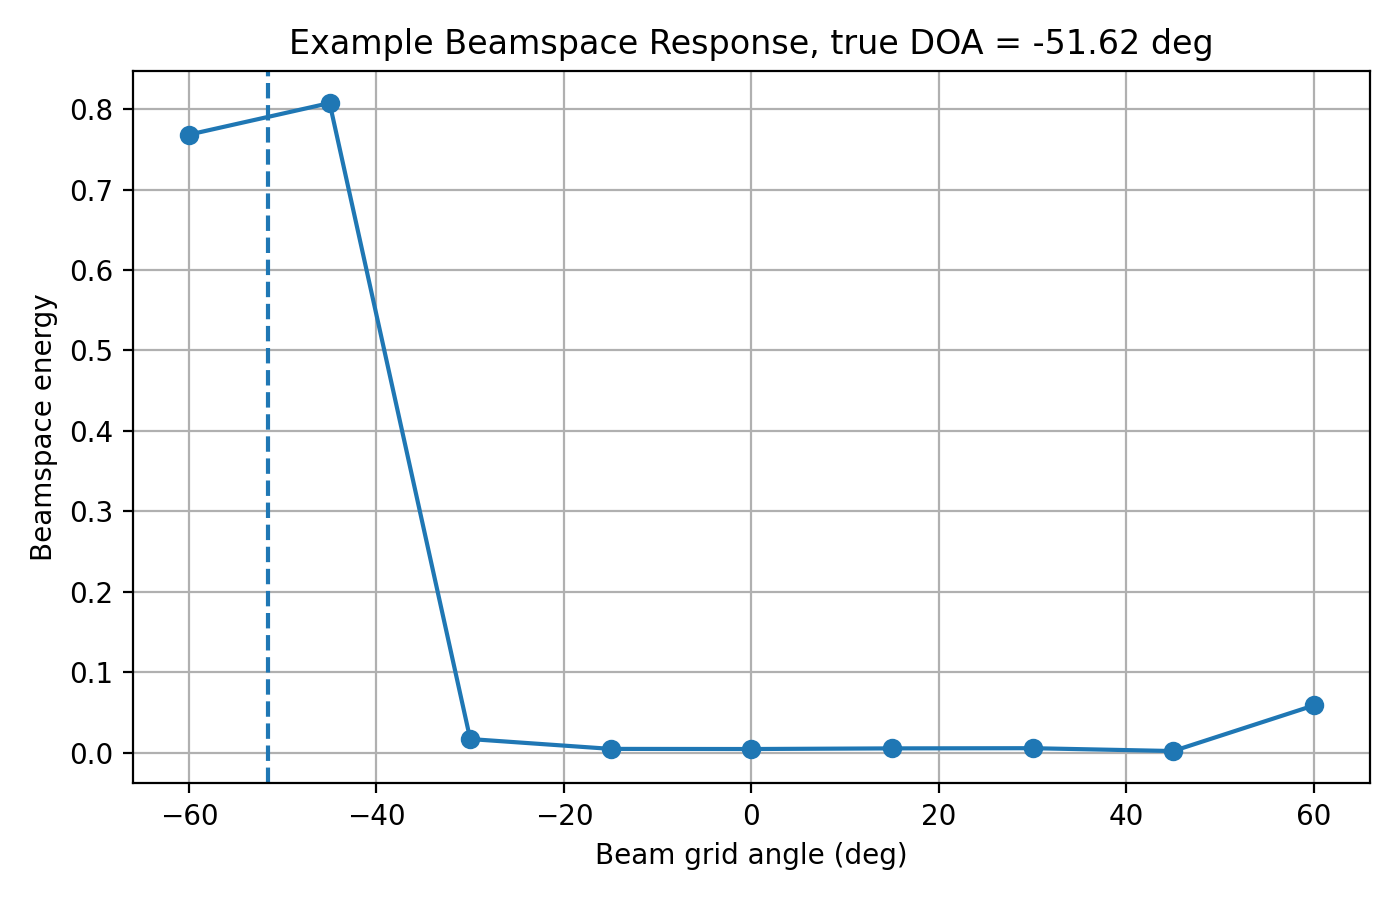
\includegraphics[width=0.78\linewidth]{run_001_example_beamspace_response.png}
\vspace{0.1cm}

\small Beamspace features provide compact spatial information for coarse DOA-sector classification.
\end{frame}

\begin{frame}{Baseline and LIF Inference}
\begin{columns}
\column{0.48\textwidth}
\textbf{Nearest-centroid baseline}
\begin{itemize}
    \item Continuous normalized features.
    \item Deterministic and interpretable.
    \item Overall accuracy: $0.869048$.
\end{itemize}
\column{0.48\textwidth}
\textbf{LIF-inspired classifier}
\begin{itemize}
    \item Rate-coded spike trains.
    \item Leaky temporal evidence accumulation.
    \item Fixed Run 003 accuracy: $0.825000$.
\end{itemize}
\end{columns}
\end{frame}

\begin{frame}{LIF Temporal Accumulation}
\begin{equation*}
    v_c[t] = \alpha v_c[t-1] + i_c[t]
\end{equation*}
\begin{itemize}
    \item $v_c[t]$: membrane evidence for class $c$.
    \item $\alpha$: leak factor.
    \item $i_c[t]$: spike-driven input current.
    \item Stable-decision latency is the earliest time after which the final decision remains unchanged.
\end{itemize}
\begin{block}{Fixed Run 003}
$T=20$, leak $=0.97$, accuracy $=0.825000$, mean latency $=6.423810$ time steps.
\end{block}
\end{frame}

\begin{frame}{Accuracy Comparison}
\centering
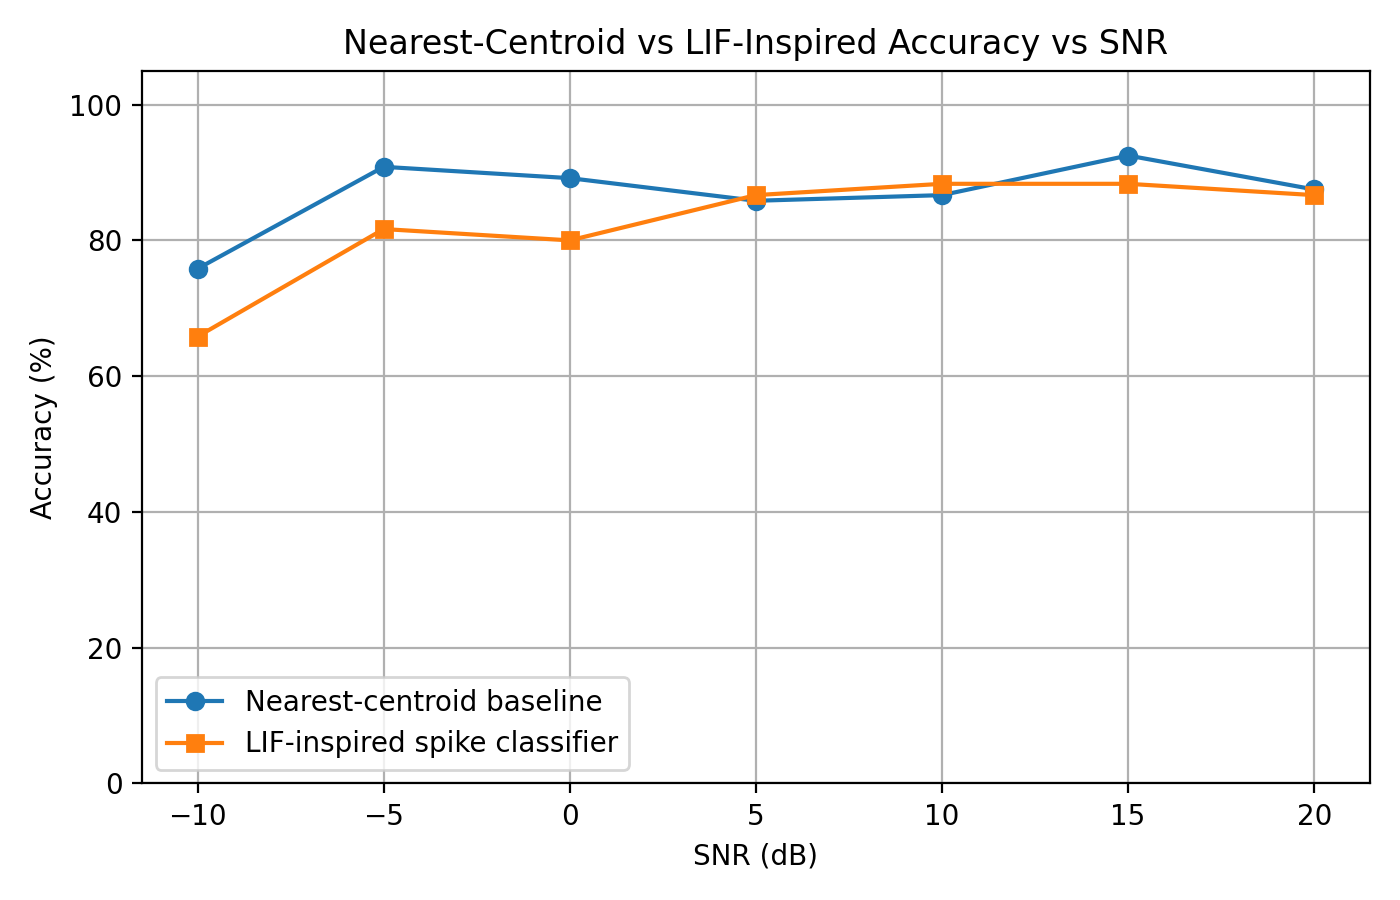
\includegraphics[width=0.82\linewidth]{run_004_accuracy_comparison_vs_snr.png}
\vspace{0.1cm}

\small The LIF-inspired classifier remains below the continuous baseline but well above the four-class random baseline.
\end{frame}

\begin{frame}{Latency Versus SNR}
\centering
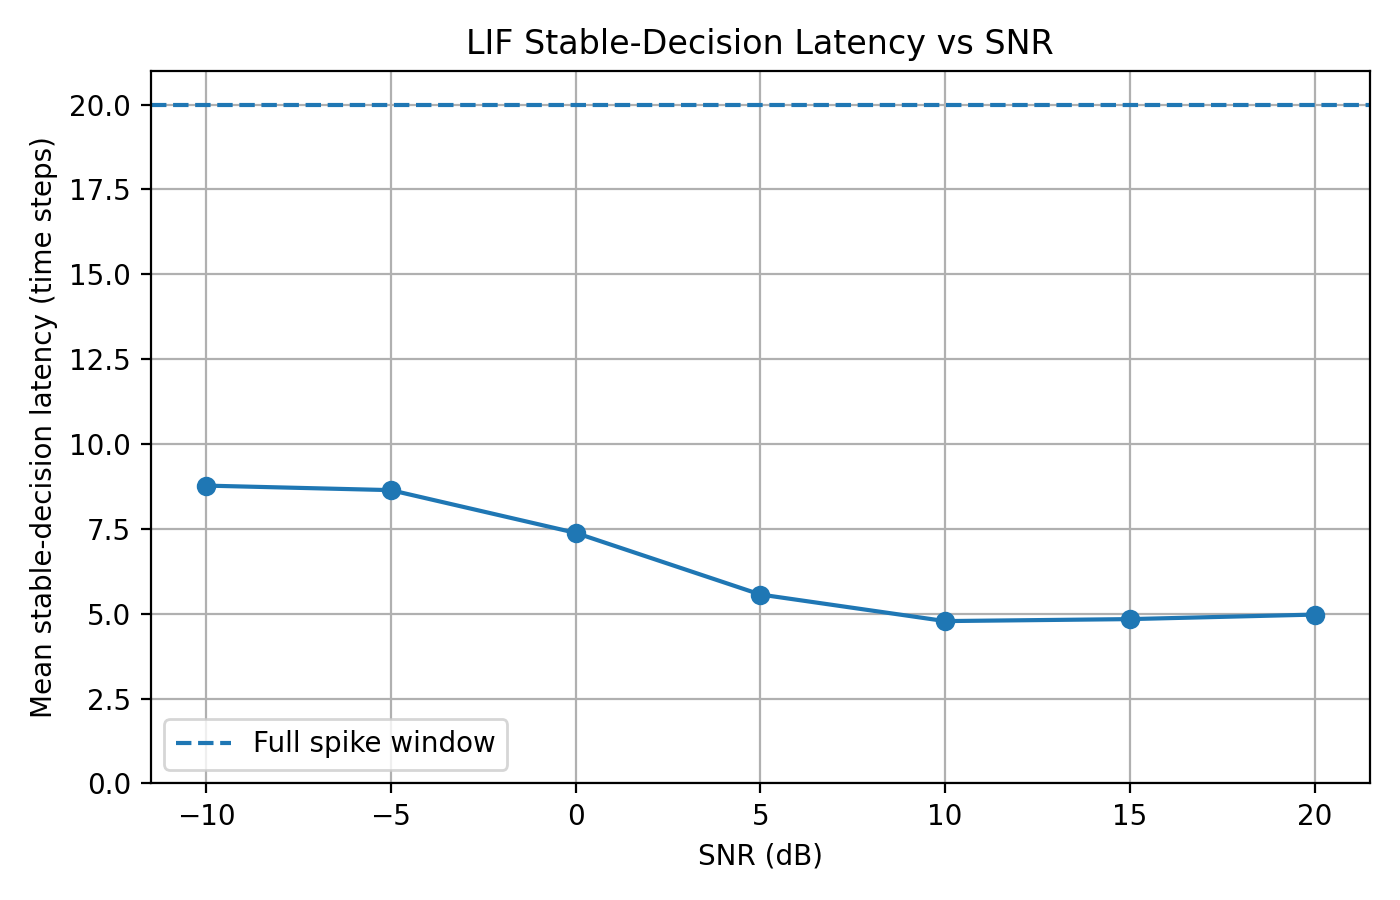
\includegraphics[width=0.82\linewidth]{run_004_lif_latency_vs_snr.png}
\vspace{0.1cm}

\small Higher signal quality generally stabilizes the temporal decision earlier.
\end{frame}

\begin{frame}{Run 005 Parameter Sweep}
\centering
\begin{tabular}{lrrrr}
\toprule
Case & $T$ & Leak & Accuracy & Latency \\
\midrule
Best LIF accuracy & 40 & 0.99 & 0.841667 & 8.396429 \\
Lowest latency & 10 & 0.99 & 0.776190 & 3.782143 \\
Fixed Run 003 & 20 & 0.97 & 0.825000 & 6.423810 \\
Baseline & -- & -- & 0.869048 & -- \\
\bottomrule
\end{tabular}
\vspace{0.3cm}

\small The sweep exposes a direct accuracy--latency design trade-off.
\end{frame}

\begin{frame}{Accuracy--Latency Trade-Off}
\centering
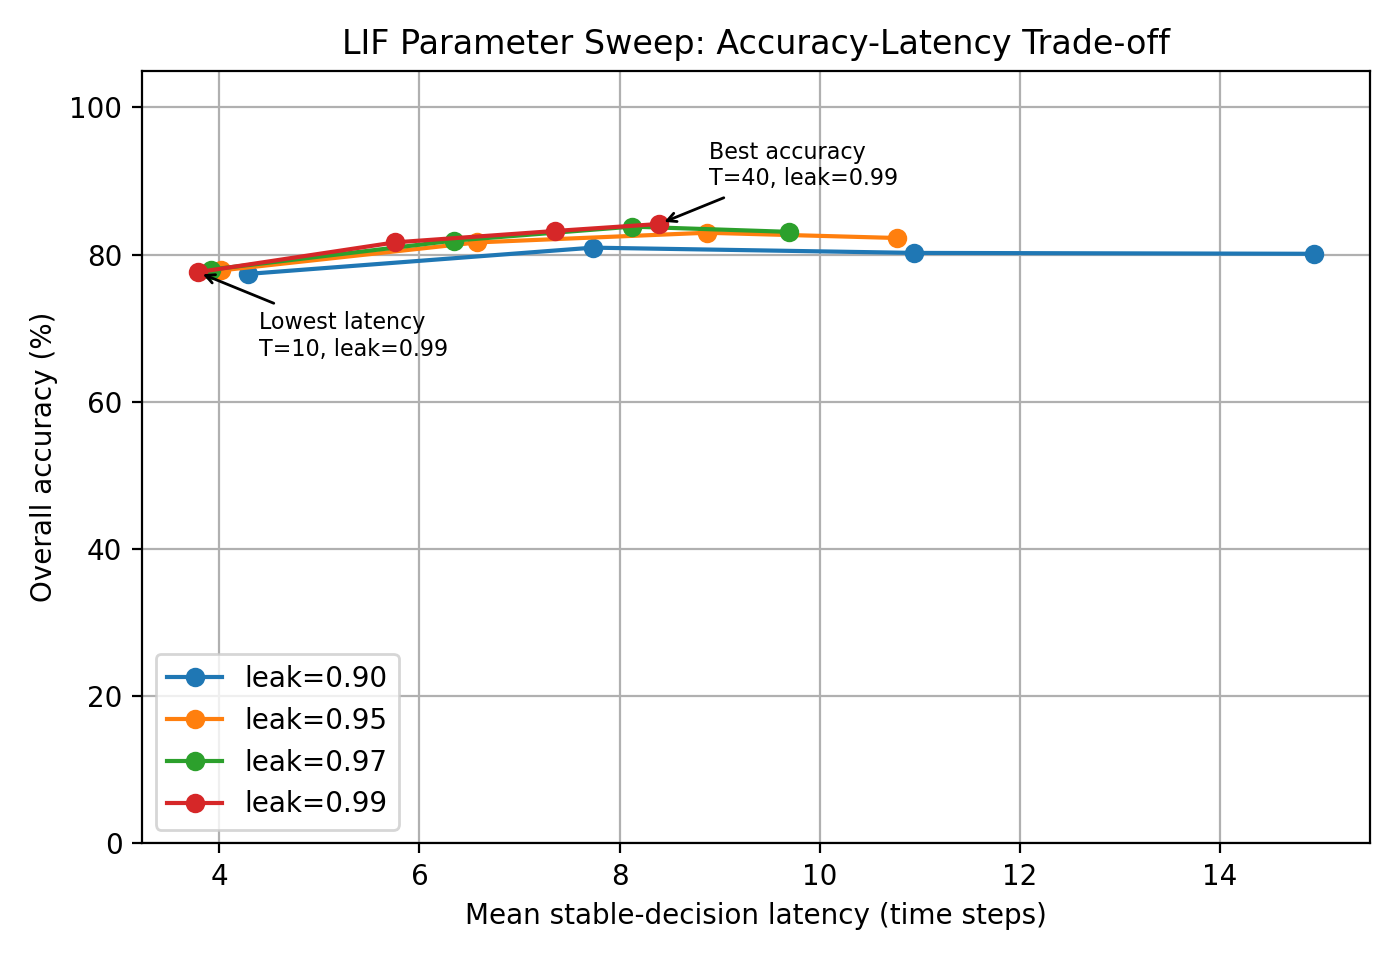
\includegraphics[width=0.80\linewidth]{run_005_lif_accuracy_latency_tradeoff.png}
\vspace{0.1cm}

\small Longer spike windows and stronger evidence retention improve accuracy but increase temporal budget.
\end{frame}

\begin{frame}{Engineering Interpretation}
\begin{itemize}
    \item Beamspace features are informative for coarse DOA-sector inference.
    \item Spike encoding introduces some accuracy loss but enables sparse temporal processing.
    \item LIF parameters provide explicit control over the accuracy--latency trade-off.
    \item Phase 1 is a stable reference model for embedded implementation and hardware-aware refactoring.
\end{itemize}
\end{frame}

\begin{frame}{Conclusion and Next Steps}
\begin{block}{Conclusion}
Phase 1 successfully establishes an end-to-end DOA/SNN reference prototype with reproducible metrics, figures, and documentation.
\end{block}
\begin{itemize}
    \item Finalize course report package.
    \item Extend toward richer radar/DOA case studies.
    \item Refactor selected kernels for PYNQ or Vitis HLS.
\end{itemize}
\end{frame}

\end{document}
